\chapter{Metodología}

\section{Diseño de investigación}
Este estudio corresponde a un diseño de investigación aplicada y de desarrollo tecnológico, enfocado en la creación e implementación de una aplicación web responsive que integra APIs de inteligencia artificial generativa para apoyar el desarrollo del habla en niños con Síndrome de Down. La metodología combina fases de desarrollo software full-stack con pruebas funcionales para validar la integración y efectividad de los componentes tecnológicos.

\section{Participantes}
Como se trata de un proyecto de desarrollo de software, no se contó con participantes humanos durante la fase de desarrollo. La aplicación está dirigida a terapeutas del habla, padres y niños con Síndrome de Down del contexto latinoamericano, quienes serán los usuarios finales de la herramienta.

\section{Instrumentos}
Los principales instrumentos y herramientas utilizados en este proyecto incluyen:
\begin{itemize}
    \item Tecnologías backend: Node.js con Express, Sequelize para ORM, PostgreSQL como sistema gestor de base de datos.
    \item Tecnologías frontend: React.js con Tailwind CSS para el diseño responsive y accesible.
    \item APIs externas: OpenAI para generación de contenido con IA, Google Cloud Text-to-Speech para generación de audio.
    \item Herramientas de prueba y desarrollo: Postman para pruebas de APIs REST, entornos de desarrollo integrados y control de versiones.
\end{itemize}

\section{Procedimiento}
El desarrollo del proyecto se realizó siguiendo los siguientes pasos:

\begin{enumerate}

\item Creación de la estructura de carpetas raíz para backend y frontend, para organizar el código y los recursos del proyecto.

\vspace{0.5cm}
\begin{figure}[H]
    \centering
    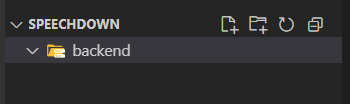
\includegraphics[width=0.8\textwidth]{imagenes/estructura_carpetas.png}
    \caption{Estructura de carpetas del proyecto SpeechDown}
    \label{fig:estructura_carpetas}
\end{figure}
\vspace{0.5cm}

\item Inicialización del proyecto Node.js en la carpeta backend e instalación de dependencias necesarias para servidor, conexión con APIs externas y manejo de base de datos.

\vspace{0.5cm}
\begin{figure}[H]
    \centering
    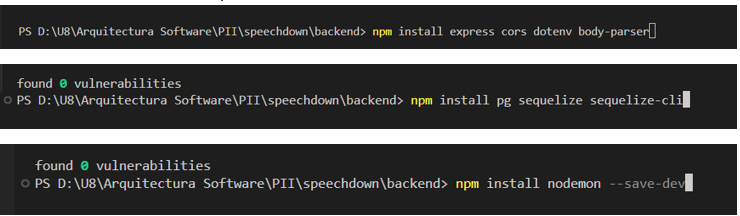
\includegraphics[width=0.8\textwidth]{imagenes/instalacion_dependencias_backend.png}
    \caption{Instalación de dependencias en backend}
    \label{fig:instalacion_dependencias_backend}
\end{figure}
\vspace{0.5cm}

\item Configuración inicial del archivo \texttt{app.js} para establecer el servidor Express y definir las rutas básicas del backend.

\vspace{0.5cm}
\begin{figure}[H]
    \centering
    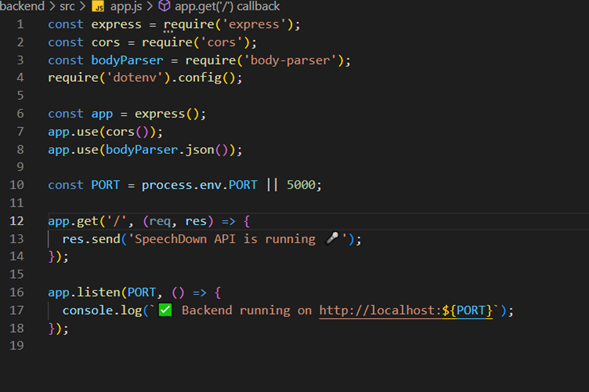
\includegraphics[width=0.8\textwidth]{imagenes/configuracion_appjs.png}
    \caption{Configuración inicial del archivo app.js}
    \label{fig:configuracion_appjs}
\end{figure}
\vspace{0.5cm}

\item Configuración y puesta en marcha del frontend con React.js, instalación de dependencias y configuración inicial en \texttt{App.jsx}.

\vspace{0.5cm}
\begin{figure}[H]
    \centering
    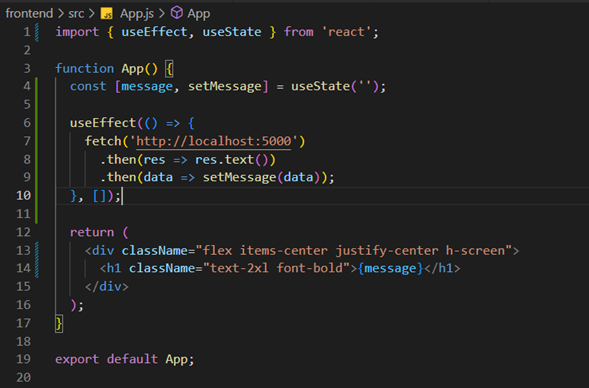
\includegraphics[width=0.8\textwidth]{imagenes/configuracion_frontend.png}
    \caption{Configuración inicial del frontend React.js}
    \label{fig:configuracion_frontend}
\end{figure}
\vspace{0.5cm}

\item Definición de la estructura interna de carpetas para backend (controladores, servicios, modelos, rutas) y frontend (componentes, páginas, servicios, assets).

\vspace{0.5cm}
\begin{figure}[H]
    \centering
    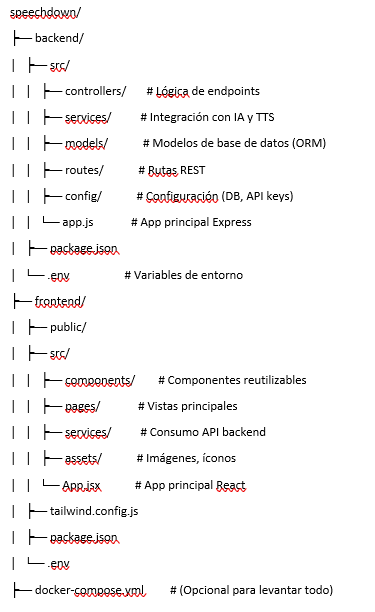
\includegraphics[width=0.8\textwidth]{imagenes/estructura_interna.png}
    \caption{Estructura interna del proyecto}
    \label{fig:estructura_interna}
\end{figure}
\vspace{0.5cm}

\item Ejecución simultánea del backend y frontend en terminales independientes para verificar comunicación y funcionamiento básico.

\vspace{0.5cm}
\begin{figure}[H]
    \centering
    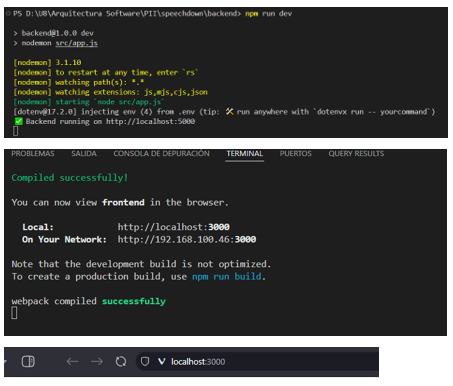
\includegraphics[width=0.8\textwidth]{imagenes/ejecucion_terminales.png}
    \caption{Ejecución de backend y frontend}
    \label{fig:ejecucion_terminales}
\end{figure}
\vspace{0.5cm}

\item Creación y configuración de la base de datos PostgreSQL “speechdown” y configuración de Sequelize como ORM para manipulación de datos.

\vspace{0.5cm}
\begin{figure}[H]
    \centering
    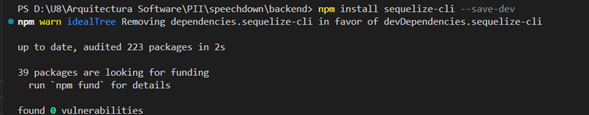
\includegraphics[width=0.8\textwidth]{imagenes/configuracion_postgresql.png}
    \caption{Configuración de PostgreSQL y Sequelize}
    \label{fig:configuracion_postgresql}
\end{figure}
\vspace{0.5cm}

\item Definición y creación de los modelos de datos: usuario, niño y actividad.

\vspace{0.5cm}
\begin{figure}[H]
    \centering
    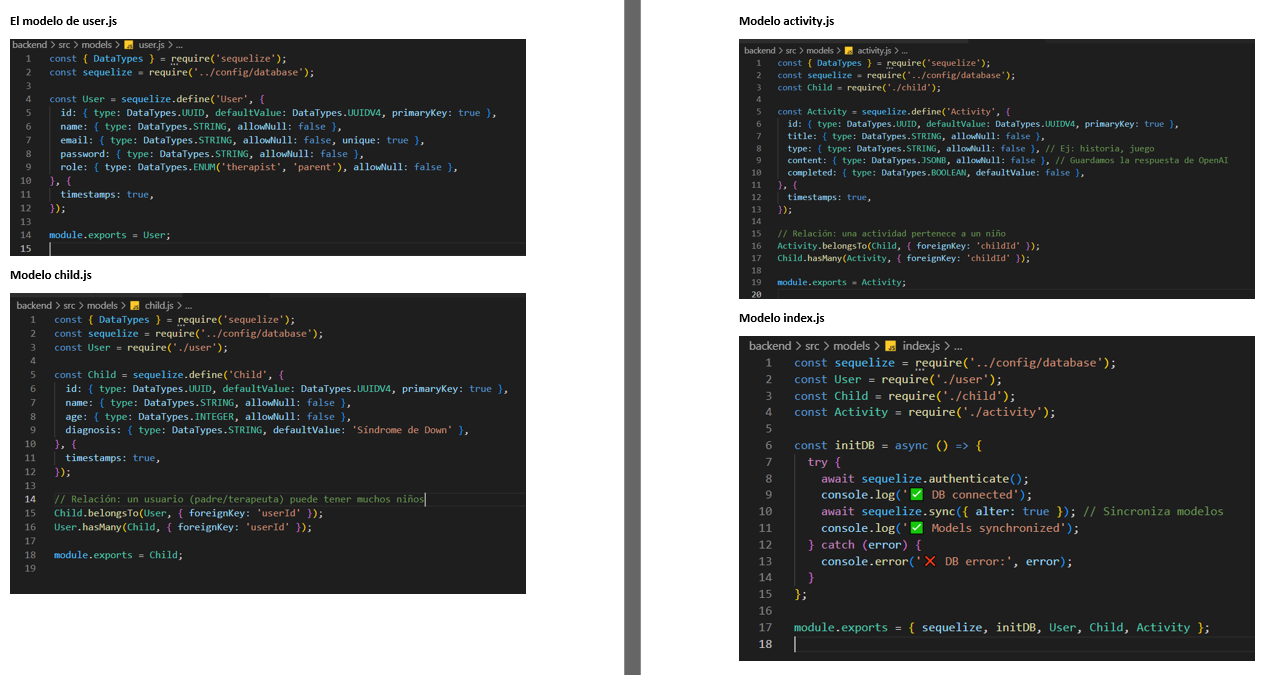
\includegraphics[width=0.8\textwidth]{imagenes/modelos_datos.png}
    \caption{Modelos de datos definidos para la aplicación}
    \label{fig:modelos_datos}
\end{figure}
\vspace{0.5cm}

\item Validación del correcto funcionamiento del backend y verificación de la creación de tablas en la base de datos.

\vspace{0.5cm}
\begin{figure}[H]
    \centering
    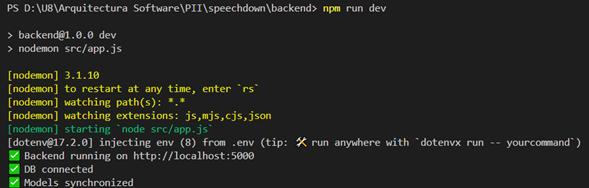
\includegraphics[width=0.8\textwidth]{imagenes/validacion_backend.png}
    \caption{Validación del backend y tablas en base de datos}
    \label{fig:validacion_backend}
\end{figure}
\vspace{0.5cm}

\item Integración de la API de OpenAI para la generación de ejercicios personalizados mediante IA.

\vspace{0.5cm}
\begin{figure}[H]
    \centering
    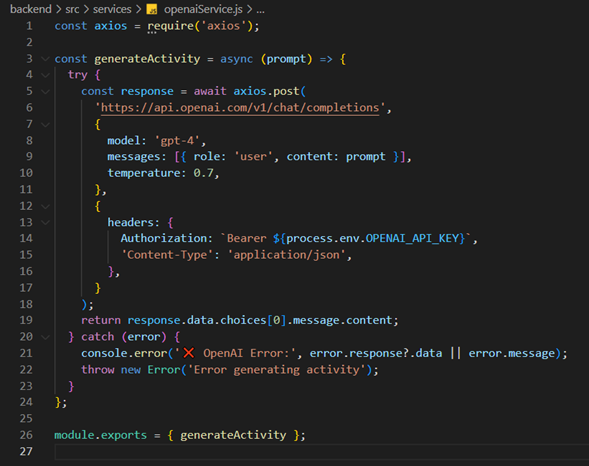
\includegraphics[width=0.8\textwidth]{imagenes/integracion_openai.png}
    \caption{Integración con API de OpenAI}
    \label{fig:integracion_openai}
\end{figure}
\vspace{0.5cm}

\item Desarrollo de controladores y rutas para manejo de actividades generadas por IA, con pruebas mediante Postman.

\vspace{0.5cm}
\begin{figure}[H]
    \centering
    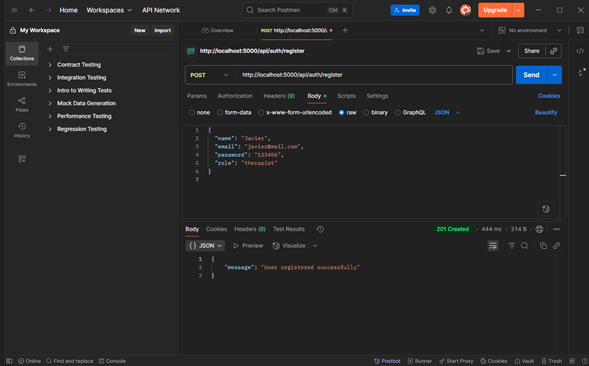
\includegraphics[width=0.8\textwidth]{imagenes/pruebas_postman.png}
    \caption{Pruebas de API con Postman}
    \label{fig:pruebas_postman}
\end{figure}
\vspace{0.5cm}

\item Integración del servicio Google Cloud Text-to-Speech (TTS), configuración de cuenta, instalación de dependencias y creación de endpoints para generación y almacenamiento de audios.

\vspace{0.5cm}
\begin{figure}[H]
    \centering
    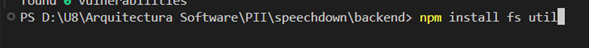
\includegraphics[width=0.8\textwidth]{imagenes/integracion_tts.png}
    \caption{Integración con Google Text-to-Speech}
    \label{fig:integracion_tts}
\end{figure}
\vspace{0.5cm}

\item Implementación del sistema de autenticación de usuarios (registro y login) con pruebas desde Postman.

\vspace{0.5cm}
\begin{figure}[H]
    \centering
    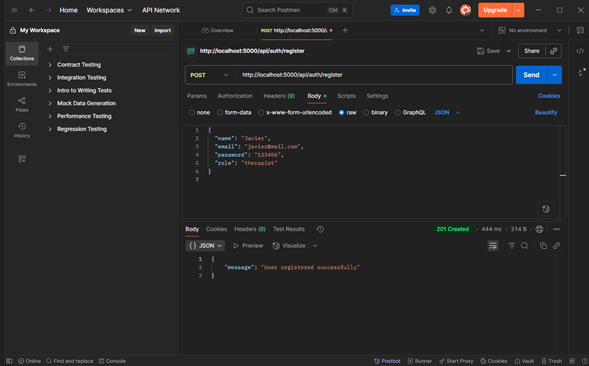
\includegraphics[width=0.8\textwidth]{imagenes/autenticacion_usuarios.png}
    \caption{Implementación del sistema de autenticación}
    \label{fig:autenticacion_usuarios}
\end{figure}
\vspace{0.5cm}

\item Conexión del backend con el frontend para permitir la interacción de usuarios con las funcionalidades del sistema.

\vspace{0.5cm}
\begin{figure}[H]
    \centering
    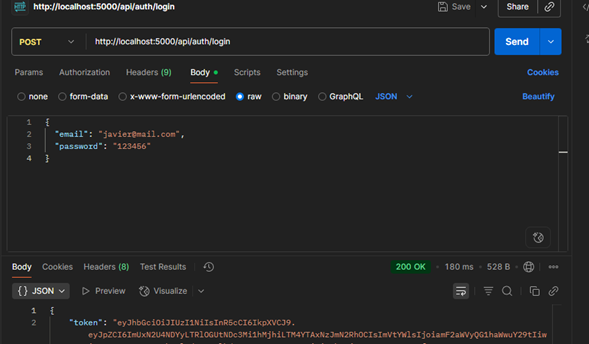
\includegraphics[width=0.8\textwidth]{imagenes/conexion_backend_frontend.png}
    \caption{Conexión entre backend y frontend}
    \label{fig:conexion_backend_frontend}
\end{figure}
\vspace{0.5cm}

\item Desarrollo de la interfaz gráfica para la gestión de usuarios y asignación de niños a terapeutas o padres.

\vspace{0.5cm}
\begin{figure}[H]
    \centering
    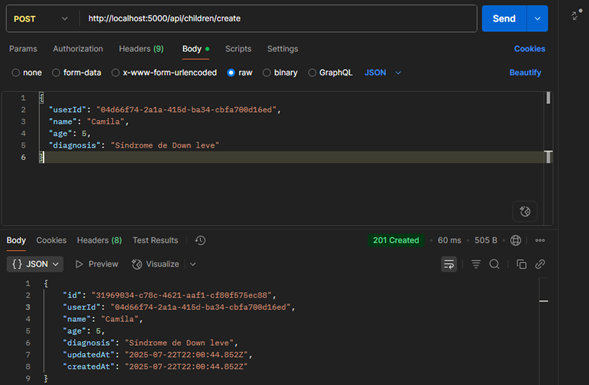
\includegraphics[width=0.8\textwidth]{imagenes/interfaz_gestion_usuarios.png}
    \caption{Interfaz gráfica para gestión de usuarios y niños}
    \label{fig:interfaz_gestion_usuarios}
\end{figure}
\vspace{0.5cm}

\item Creación, gestión y prueba de actividades interactivas generadas mediante IA, validando integración con APIs OpenAI y TTS.

\vspace{0.5cm}
\begin{figure}[H]
    \centering
    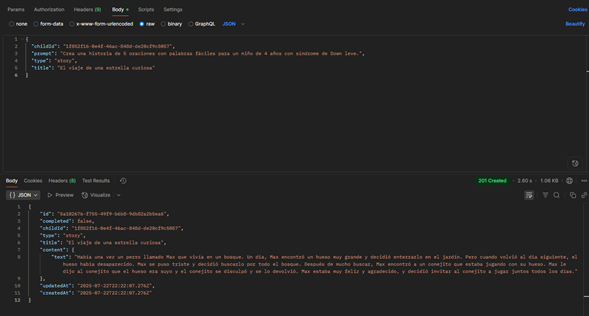
\includegraphics[width=0.8\textwidth]{imagenes/gestion_actividades.png}
    \caption{Gestión y creación de actividades interactivas}
    \label{fig:gestion_actividades}
\end{figure}
\vspace{0.5cm}

\item Realización de pruebas finales para verificar la correcta generación de audios y visualización de datos en la interfaz gráfica.

\vspace{0.5cm}
\begin{figure}[H]
    \centering
    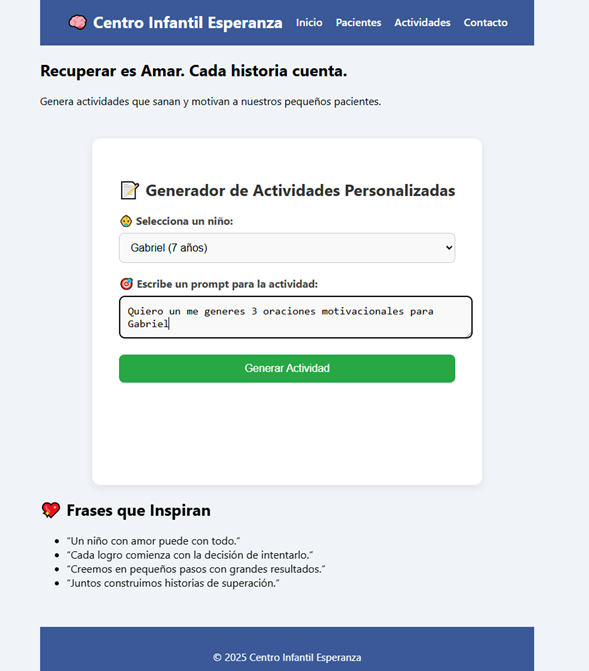
\includegraphics[width=0.8\textwidth]{imagenes/pruebas_finales.png}
    \caption{Pruebas finales y verificación de generación de audios}
    \label{fig:pruebas_finales}
\end{figure}
\vspace{0.5cm}

\end{enumerate}
